\documentclass{article}
\usepackage{listings}
\usepackage{xcolor}
\usepackage{aligned-overset}
\usepackage{bookmark}
\usepackage{fancyhdr}
\usepackage{array}
\usepackage{appendix}
\usepackage{xcolor}
\usepackage{bm}
\usepackage{chapterbib}
\usepackage{float}
\usepackage[UTF8]{ctex}
\usepackage{geometry}
%\geometry{a4paper,scale=0.8}
\pagestyle{fancy}
\fancyhf{}
%\fancyhead[C]{ACM模板 by 嘤嘤嘤} %页眉与页脚
%\fancyfoot[C]{} 
\rfoot{\thepage} % 显示页码
%\hypersetup{hidelinks} % 隐藏目录红色边框

\newfontfamily\codeFont{SourceCodePro-Medium}
\newfontfamily\codeBold{SourceCodePro-Bold}
\newfontfamily\commentFont{Courier Regular}


\usepackage{chapterbib}
\usepackage{xltxtra}
\usepackage{geometry}
\usepackage{natbib}
\usepackage{url}
\usepackage{graphicx}
\renewcommand\arraystretch{2}
\usepackage{subfigure}
\usepackage{enumerate}
\geometry{left=2.18cm,right=2.08cm,top=1.84cm,bottom=1.84cm}
\usepackage{graphicx}
\usepackage{listings}
\pagestyle{plain}   
\usepackage{setspace}
\usepackage{indentfirst}
\usepackage{caption2}
\usepackage{datetime} %日期
\renewcommand{\today}{\number\year 年 \number\month 月 \number\day 日}
\renewcommand{\captionlabelfont}{\small}
\renewcommand{\captionfont}{\small}
\usepackage{pythonhighlight}
\setlength{\parindent}{2em}
\lstset{language=Matlab}%代码语言使用的是matlab

\lstset{breaklines}%自动将长的代码行换行排版
\lstset{
    language    = c++,
    numbers     = left,
    numberstyle = \small,
    breaklines  = true,
    captionpos  = b,
    tabsize     = 4,
%   frame       = shadowbox,
    frame       = leftline,
    columns     = fullflexible,
    commentstyle = \commentFont\color[RGB]{0,0,0},
    keywordstyle = \codeBold\color[RGB]{0,0,0},
    basicstyle   = \small\codeFont,
    stringstyle  = \color[RGB]{48,0,20}\codeFont,
    rulesepcolor = \color{red!20!green!20!blue!20},
    showstringspaces = false,
}
\lstset{extendedchars=false}%解决代码跨页时,章节标题,页眉等汉字不显示的问题
\title{基于SIR模型对武汉新型冠状病毒疫情分析} 
\date{} 
\begin{document}
\begin{figure}
    
\includegraphics[width=8cm]{upc.png}

    \label{figupc}
\end{figure}

  \begin{center}
    \quad \\
    \quad \\
    \heiti \fontsize{45}{17} \quad \quad \quad 
    \vskip 1.5cm
    \heiti \zihao{2} 互联网邮件收发程序设计
  \end{center}
  \vskip 2.0cm
    
  \begin{quotation}
%   \begin{center}
    \doublespacing
    
        \zihao{4}\par\setlength\parindent{7em}
    \qquad 

    学生姓名:\underline{\qquad  张世琛 \qquad \qquad}

    学\hspace{0.61cm} 号:\underline{\qquad 1804030401\qquad}
    
    专业班级:\underline{\qquad 计科1802 \qquad  }
    
    学\hspace{0.61cm} 院:\underline{计算机科学与技术学院}
%   \end{center}
    \vskip 1cm
    \centering
    \begin{table}[h]
            \centering 
            \zihao{4}
            \begin{tabular}{|p{3.5cm}<{\centering}|p{9cm}<{\centering}|}
            % 这里的rl 与表格对应可以看到,姓名是r,右对齐的;学号是l,左对齐的;若想居中,使用c关键字。
                \hline
                实验成绩 & \\ [6pt]
                \hline
                教师评阅& \\ [85pt]
                \hline
            \end{tabular}
        \end{table}
    \vskip 1cm
    \today
  \end{quotation}
\thispagestyle{empty}
\newpage
\setcounter{page}{1}
\songti\zihao{4}
\section{实验目的}
\begin{enumerate}
    \item 熟练掌握通过 Linux Socket 编程实现 SMTP、POP3 命令字的交互。
    \item 开发出收发邮件的程序。
    \item 设计邮件收发程序的流程图。
\end{enumerate}
\section{环境要求}
\begin{enumerate}
    \item 硬件要求: \\
    PC 机; 
    \item 软件环境: \\
    VMware 虚拟机;Linux 操作系统;MAIL 服务器环境;vi 编辑器 或 gedit 文本编辑器;gcc 编译环境; 
\end{enumerate}
\section{实验内容}
\subsection{查看MAIL服务器的安装状态,当前系统已安装sendmail,pop3,imap,m4,mailx。}
\begin{figure}[h]
    \centering
    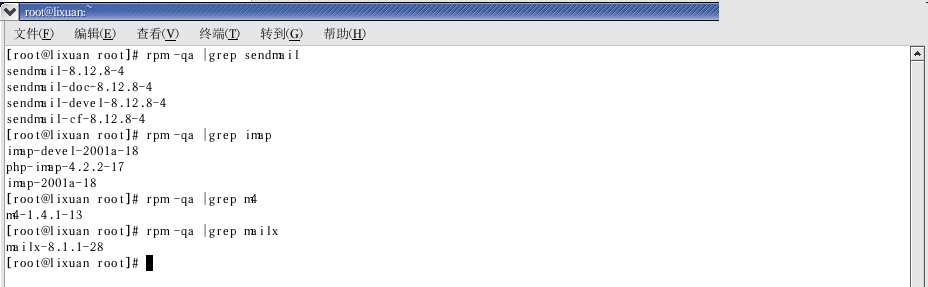
\includegraphics[width=11cm,height=4cm]{13.png}
    \caption{修改 ipop3 的文件}
\end{figure}
\subsection{在 Linux 环境下配置启动 MAIL 服务器,测试运行。}
\begin{enumerate}
\item 设置虚拟机的网络连接,如图所示\\
\begin{figure}[h]
    \centering
    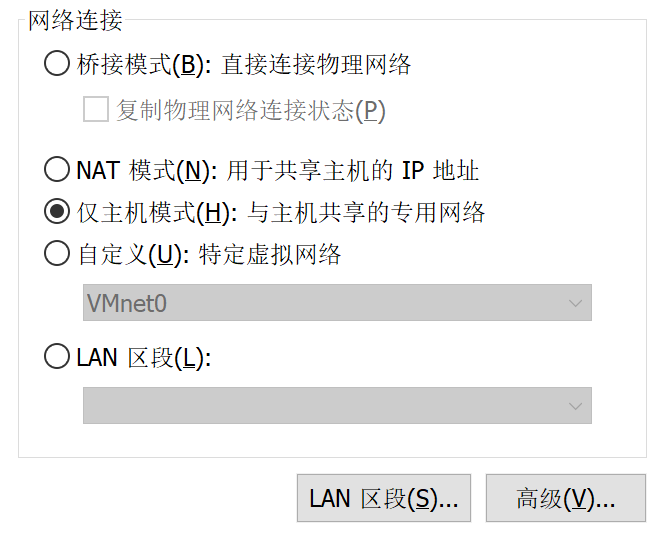
\includegraphics[width=6.5cm,height=5cm]{5.png}
    \caption{虚拟机网络连接设置}
\end{figure}
\newpage
\item 设置本地网络连接,如图所示\\
\begin{figure}[h]
    \centering
    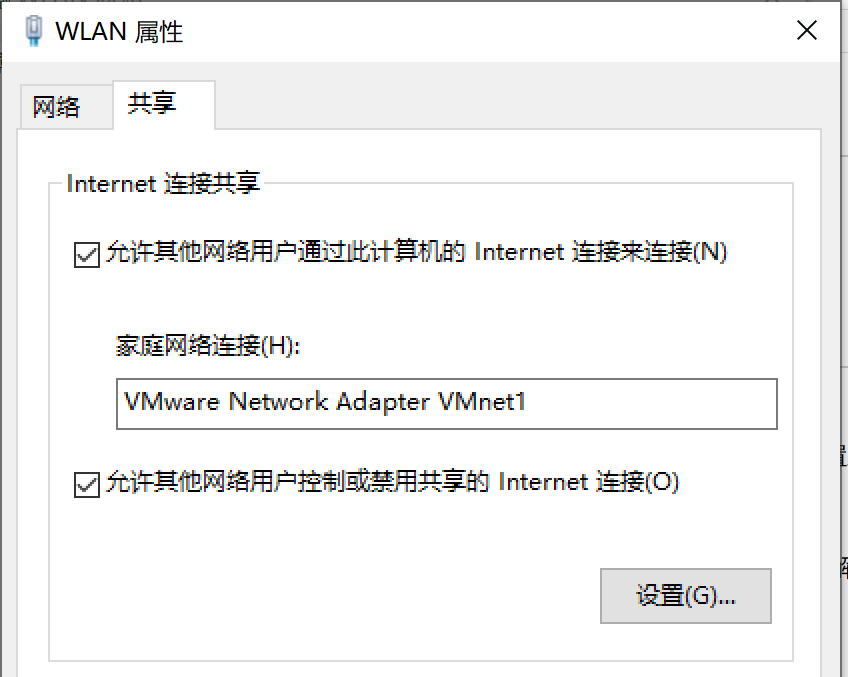
\includegraphics[width=8cm,height=6cm]{6.png}
    \caption{设置本地网络连接}
\end{figure}
\item 修改 sendmail.mc 的文件\\
\begin{figure}[h]
    \centering
    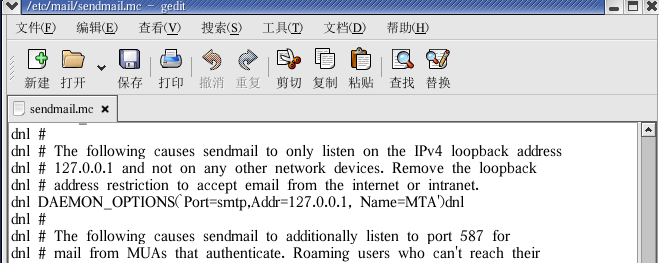
\includegraphics[width=11cm,height=4cm]{7.png}
    \caption{修改 sendmail.mc 的文件}
\end{figure}
\newpage
\item 修改 ipop3 的文件\\
\begin{figure}[h]
    \centering
    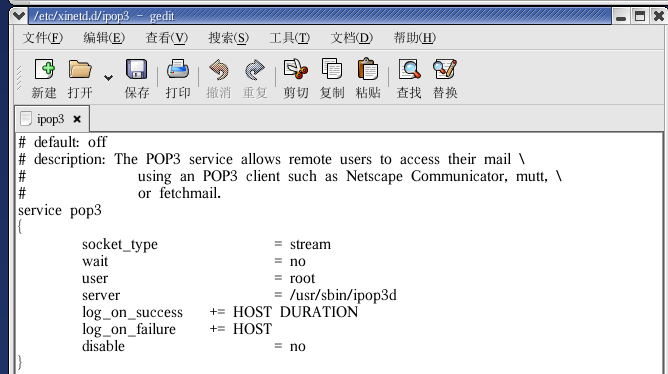
\includegraphics[width=10cm,height=4.5cm]{8.png}
    \caption{修改 ipop3 的文件}
\end{figure}
\item 输入m4 /etc/mail/sendmail.mc>/etc/mail/sendmail.cf 、 /etc/rc.d/init.d/sendmail restart、
        /etc/rc.d/init.d/senfmail restart 、/etc/rc.d/init.d/xinetd restart 命令\\
\begin{figure}[h]
    \centering
    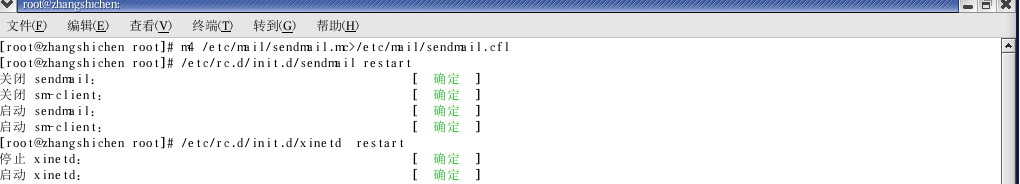
\includegraphics[width=8cm,height=2cm]{9.png}
    \caption{修改 ipop3 的文件}
\end{figure}
\item 检查pop3和smtp状态\\
\begin{figure}[h]
    \centering
    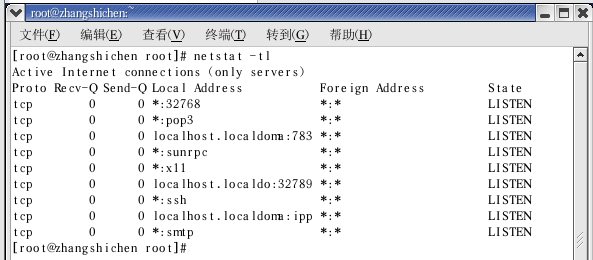
\includegraphics[width=7cm,height=3.7cm]{10.png}
    \caption{检查pop3和smtp状态}
\end{figure}

\item 在root用户下使用mail服务器发送邮件给$zhangshichen@zhangshichen.com$和$zhangshichen1@zhangshichen.com$发送邮件,\\其中$zhangshichen1@zhangshichen.com$为抄送,如下图所示:
\begin{figure}[h]
    \centering
    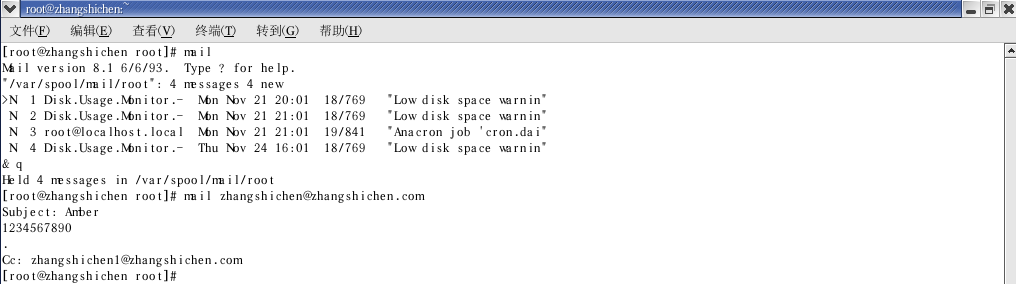
\includegraphics[width=11cm,height=4cm]{1.png}
    \caption{root用户给$zhangshichen@zhangshichen.com$和$zhangshichen1@zhangshichen.com$发送邮件}
\end{figure}
\item zhangshichen@zhangshichen.com 收到root发来的邮件
\begin{figure}[h]
    \centering
    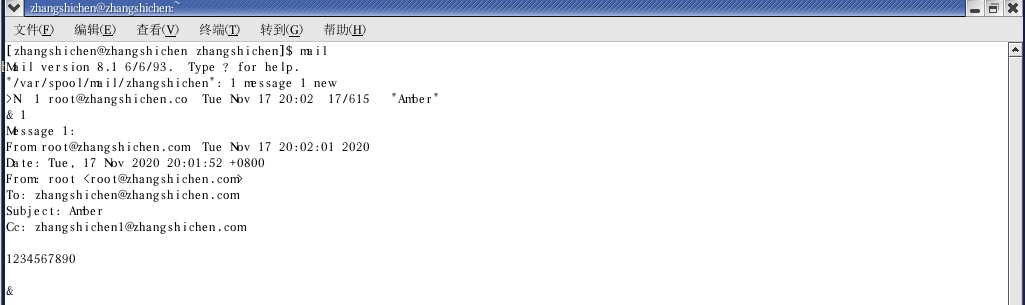
\includegraphics[width=13cm,height=4cm]{2.png}
    \caption{$zhangshichen@zhangshichen.com$收到root发来的邮件}
\end{figure}
\end{enumerate}
\subsection{使用文本编辑器编辑 SMTP 邮件发送源程序以及 POP3 接收邮件源程序,并使用 GCC 编译两个源程序分别生成可执行程序。}
\subsubsection{程序代码}
\lstinputlisting{a.cc}
\lstinputlisting{2.cc}
\subsubsection{使用文本编辑器编辑SMTP邮件发送源程序以及POP3接收邮件源程序}
\begin{figure}[h]
    \centering
    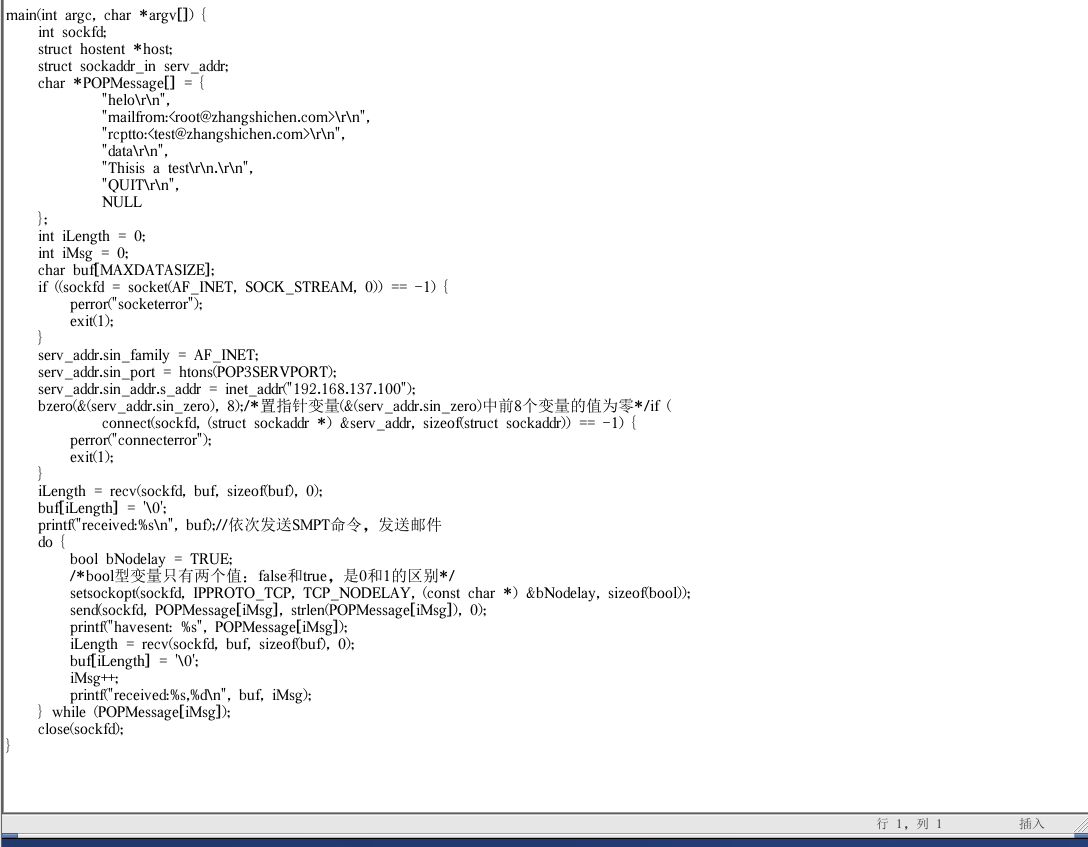
\includegraphics[width=14cm,height=10cm]{11.png}
    \caption{编写smtp程序}
\end{figure}
\begin{figure}[h]
    \centering
    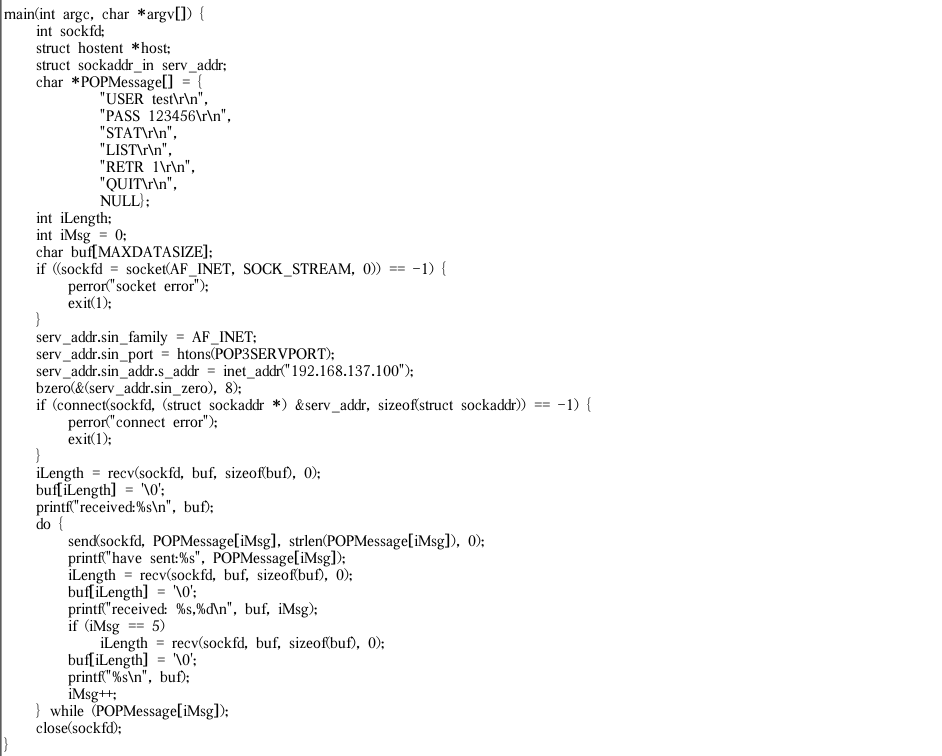
\includegraphics[width=14cm,height=10cm]{14.png}
    \caption{编写pop3程序}
\end{figure}
\newpage
\subsubsection{并使用 GCC 编译两个源程序分别生成可执行程序,并运行。}
\begin{figure}[h]
    \centering
    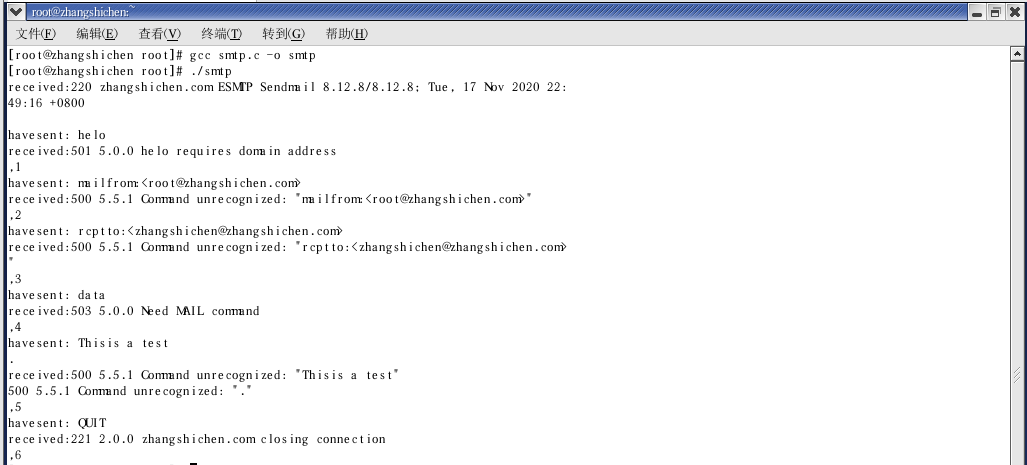
\includegraphics[width=10cm,height=5cm]{12.png}
    \caption{运行smtp程序结果}
\end{figure}
\begin{figure}[h]
    \centering
    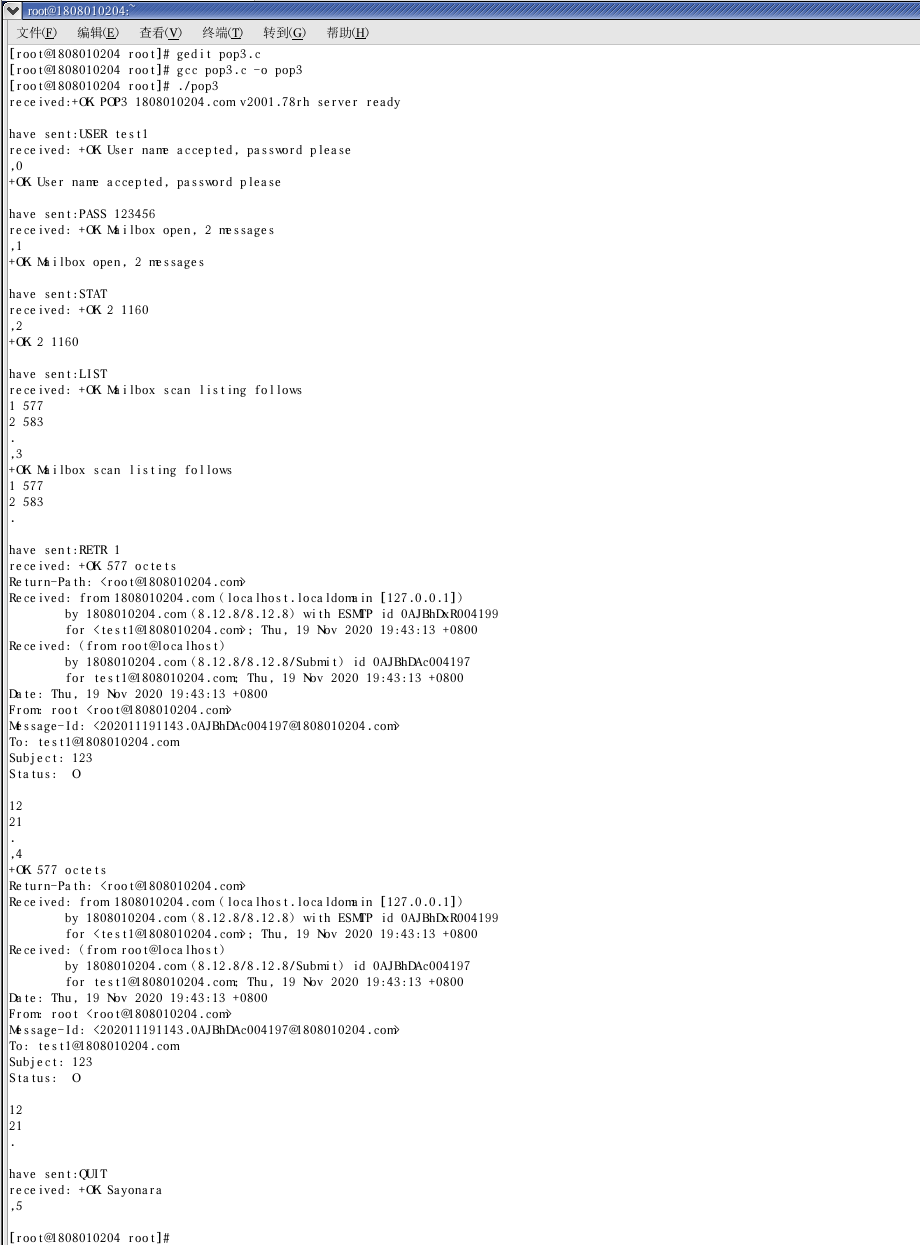
\includegraphics[width=14cm,height=16cm]{15.png}
    \caption{运行pop3程序结果}
\end{figure}
\newpage
\section{实验分析}
\subsection{SMTP通信的三个阶段的过程}
(1)连接建立,在发送主机的SMTP客户和接受主机的SMTP服务器之间建立,不使用中间的邮件服务器。

(2)邮件传送。

(3)连接释放:邮件发送完毕后,SMTP释放TCP连接。
\subsection{在电子邮件中,为什么需要使用POP和SMTP这两个协议?}
    SMTP是用来发送电子邮件的协议,POP是用来读取邮件的协议。
\subsection{IMAP与POP有什么区别?}
POP3 协议允许电子邮件客户端下载服务器上的邮件,但是在客户端的操作(如移动邮件、标记已读等),不会反馈到服务器上。\\

IMAP 提供webmail与电子邮件客户端之间的双向通信,客户端的操作都会反馈到服务器上,对邮件进行的操作,服务器上的邮件也会做相应的动作。
IMAP 整体上为用户带来更为便捷和可靠的体验。POP 更易丢失邮件或多次下载相同的邮件,但 IMAP 通过邮件客户端与webmail 之间的双向同步功能很好地避免了这些问题。
\subsection{使用SMTP、POP命令如何连接服务器?}
SMTP命令:telnet 邮件服务器名 25

POP命令:telnet  邮件服务器名  110
\subsection{发收邮件程序流程图}
\begin{figure}[htbp]
\centering
\begin{minipage}[t]{0.48\textwidth}
\centering
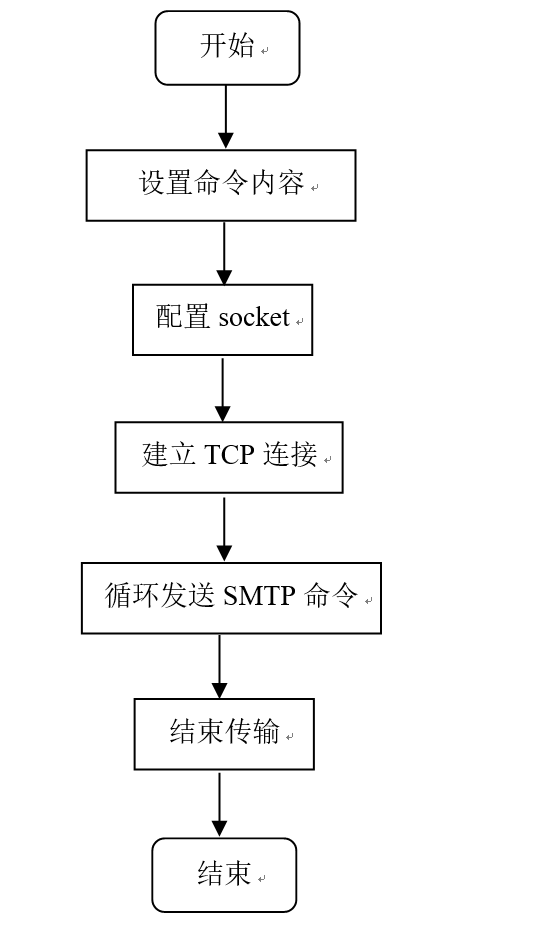
\includegraphics[height=8cm,width=6cm]{16.png}
\caption{发送邮件程序流程图}
\end{minipage}
\begin{minipage}[t]{0.48\textwidth}
\centering
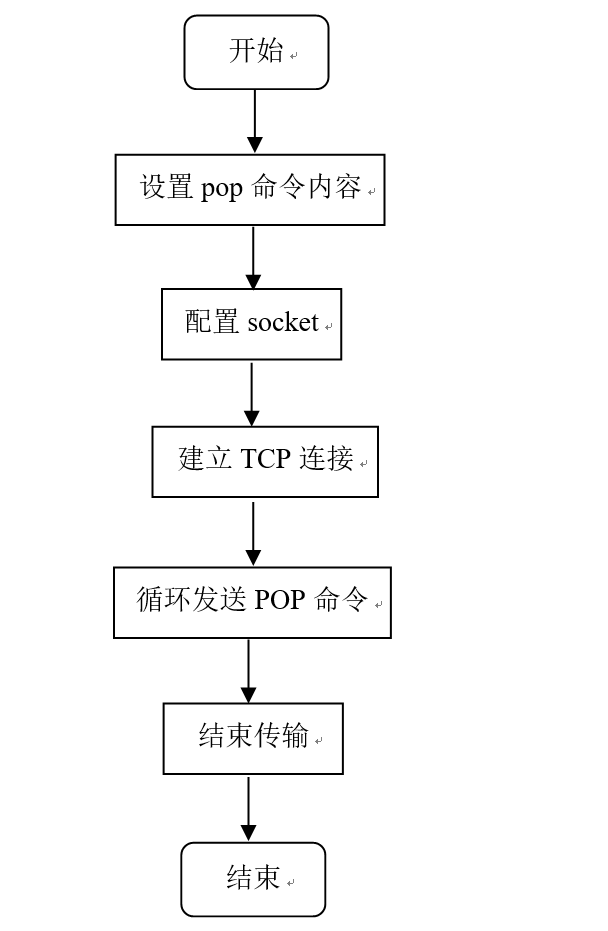
\includegraphics[height=8cm,width=6cm]{17.png}
\caption{接收邮件程序流程图}
\end{minipage}
\end{figure}
\section{实验总结}
    通过本次实验,熟悉了linux操作系统,掌握了linux环境下配置MAIL服务器的方法,学会了使用SMTP和POP命令发送和接受邮件,了解了Socket编程,通过程序编写和实际操作更加理解了电子邮件收发的工作原理和通信过程。

%\lstinputlisting{2.cc}
\end{document}

